\documentclass[10pt,a4paper]{article}
\usepackage{graphicx}

%%%%%%%%%%%%%%%%%%%%%%%%%%%
% MODIFY:

\newcommand{\authorA}{DANIEL MAYAU (03724644)}
\newcommand{\authorB}{AMELIE LASTNAME (MATRIKEL NUMBER)}
\newcommand{\authorC}{YALVAC LASTNAME (MATRIKEL NUMBER)}
\newcommand{\groupNumber}{C} % - YOUR GROUP NUMBER
\newcommand{\exerciseNumber}{1} % - THE NUMBER OF THE EXERCISE
\newcommand{\sourceCodeLink}{https:// add link}

\newcommand{\workPerAuthor}{
\authorA&Task 1&0\%\\
      &Task 2&0\%\\
      &Task 3&50\%\\
      &Task 4&80\%\\
      &Task 5&30\%\\
      \hline
\authorB&Task 1&75\%\\
      &Task 2&75\%\\
      &Task 3&50\%\\
	&Task 4&20\%\\
	&Task 5&10\%\\

      \hline
\authorC&Task 1&25\%\\
      &Task 2&25\%\\
      &Task 3&0\%\\
&Task 4&20\%\\
&Task 5&60\%\\

}

%%%%%%%%%%%%%%%%%%%%%%%%%%%

%%
% imports for the exercise sheets
%

\usepackage[utf8]{inputenc}
\usepackage{amsmath}
\usepackage{amsfonts}
\usepackage{amssymb}

\usepackage[yyyymmdd]{datetime}
\renewcommand{\dateseparator}{--}

\usepackage[left=2cm,right=2cm,top=3cm,bottom=3cm]{geometry}

\usepackage{hyperref}

\usepackage{amsthm}
\newtheorem{lem}{Lemma}
\newtheorem{thm}{Theorem}
\newtheorem{cor}{Corollary}
\newtheorem{rem}{Remark}
\newtheorem{definition}{Definition}
\newtheorem{ter}{Terminology}

\usepackage{graphicx}

\newcommand{\M}{\mathcal{M}}
\newcommand{\N}{\mathcal{N}}
\newcommand{\K}{\mathcal{K}}
\newcommand{\SPDk}{\mathbb{P}^k}
\newcommand{\vol}{\text{vol}}

\newcommand{\Figref}[1]{Figure~\ref{#1}}
\newcommand{\figref}[1]{figure~\ref{#1}}
\newcommand{\Eqnref}[1]{Equation~(\eqref{#1})}
\newcommand{\eqnref}[1]{equation~(\eqref{#1})}

\usepackage{float}
\usepackage{tabularx}

\usepackage{fancyhdr}
\pagestyle{fancy}

\usepackage{totcount}
\newtotcounter{taskCounter}
\newtotcounter{pointCounter}
\newenvironment{task}[1]{\noindent\stepcounter{taskCounter}\textbf{Report on task #1}\smallbreak\hrule\smallbreak}{\smallbreak\hrule\bigbreak}


\title{Report for exercise \exerciseNumber~from group~\groupNumber}

\makeatletter
\let\thetitle\@title
\let\theauthor\@author
\let\thedate\@date
\makeatother

\providecommand{\versiondate}{\today}

\lhead{Exercise sheet \exerciseNumber}
\chead{Master Praktikum: Modelling and Simulation of Crowds WS2019/20}
\rhead{TUM}
\lfoot{Report of Group \groupNumber}
\cfoot{\thepage}
\rfoot{Last compiled: \versiondate}
\renewcommand{\headrulewidth}{0.4pt}
\renewcommand{\footrulewidth}{0.4pt}

\newcommand{\frontpage}{
\begin{center}
\textbf{\thetitle}\\~\\
\end{center}
\begin{table}[H]
\begin{tabular}{ll}
Tasks addressed:&\total{taskCounter}\\
Authors:&\authorA\\
&\authorB\\
&\authorC\\
Last compiled:&\versiondate\\
Source code:&\sourceCodeLink
\end{tabular}
\end{table}
\vfill
The work on tasks was divided in the following way:
\begin{table}[H]
\begin{tabularx}{\textwidth}{X|p{2cm}|p{2cm}}
\workPerAuthor
\end{tabularx}
\end{table}
\newpage
}

\begin{document}

\frontpage

\begin{task}{1/5, Setting up the modeling environment}
Amelie
\end{task}

\begin{task}{2/5, First step of a single pedestrian}
§§§
Amelie \newline
§§§


\end{task}

\begin{task}{3/5, Interaction of pedestrians}
REPORT TEXT.
\end{task}

\vfill\eject





\begin{task}{4/5, Obstacle avoidance}

.\newline \newline
After pedestrian interracting with each others, the next step is to be able to avoid objects on their way. \newline
As in the following figures, the object are just runned through \newline \newline
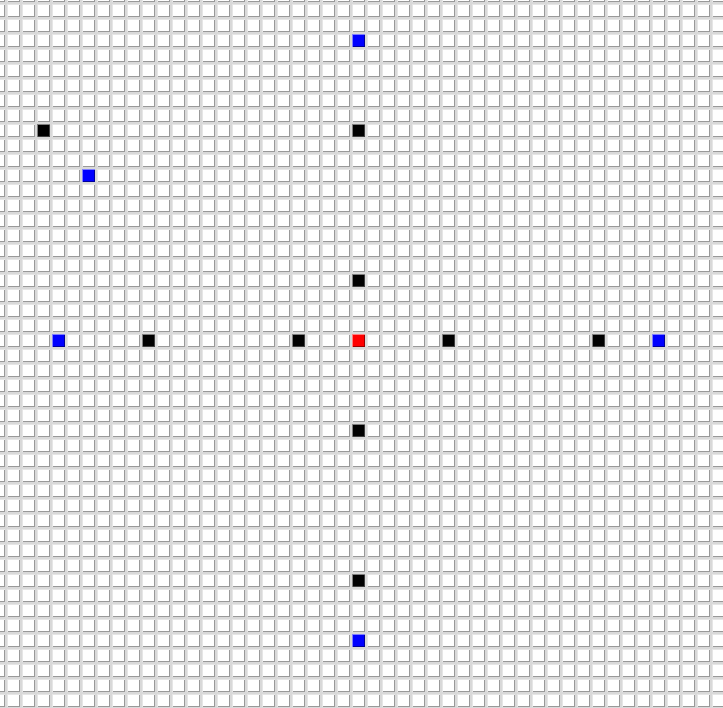
\includegraphics[height=4cm]{Travers_object_init}
~~~
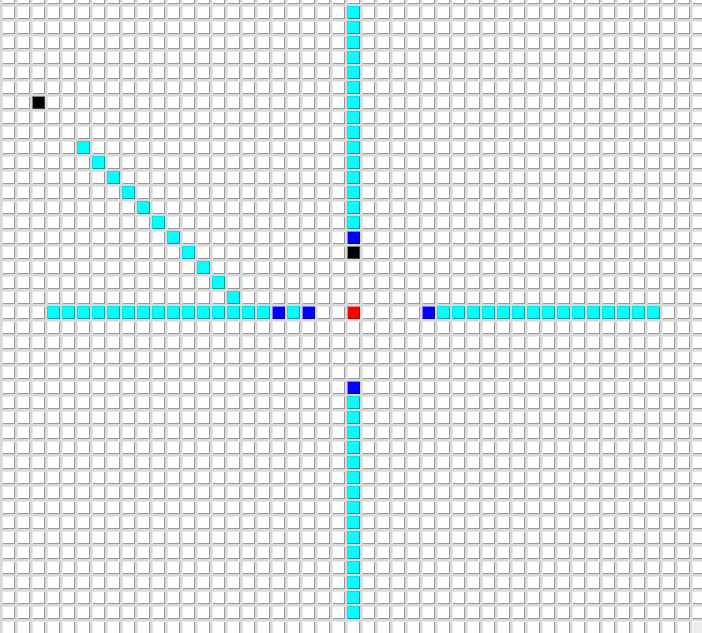
\includegraphics[height=4cm]{Travers_object_inter} \newline \newline

The first step is simply to consider obstacles to a distance infinity to the target, like it was done for the fellow pedestrians. Doing so allows us to avoid the problem of walking through the obstacles. \newline \newline
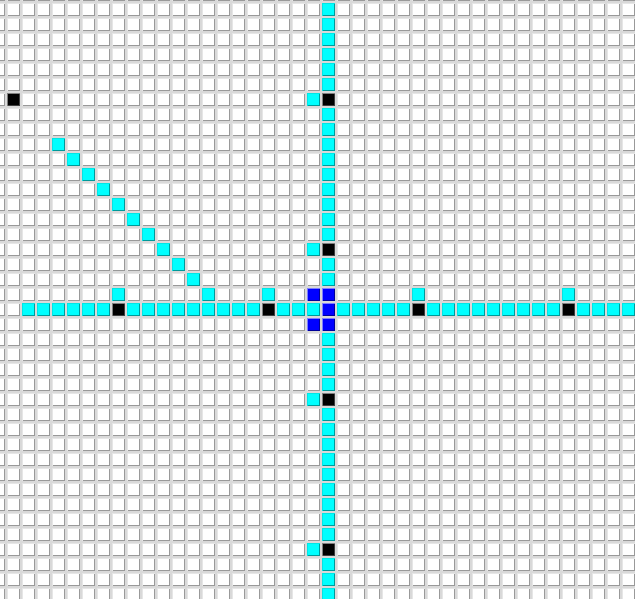
\includegraphics[height=4cm]{Travers_object_success}\newline \newline

Nevertheless this implimentation is unsuffiscient to reach the target at any time. Indeed the implementation of the Chicken Test (following figures) shows that even though the pedestrian does not go through the obstacle, it gets stuck at the obstacle, for 15 moves in the figure but potentially forever. Therefore it is important to find another way to guide the pedestrian to its goal. \newline \newline
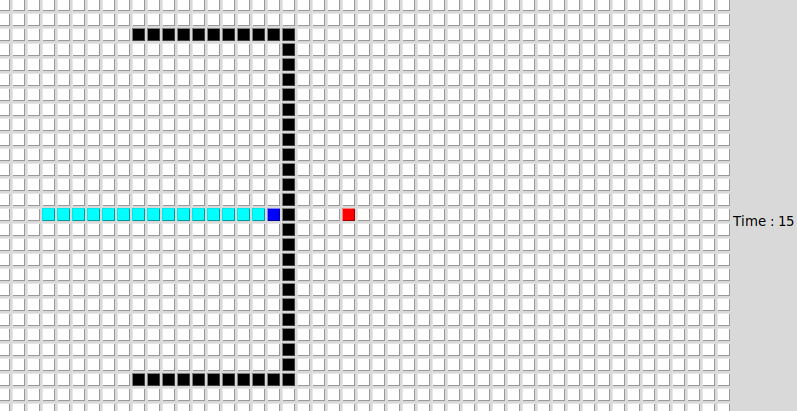
\includegraphics[height=4cm]{chicken_fail_arrival}
~~~
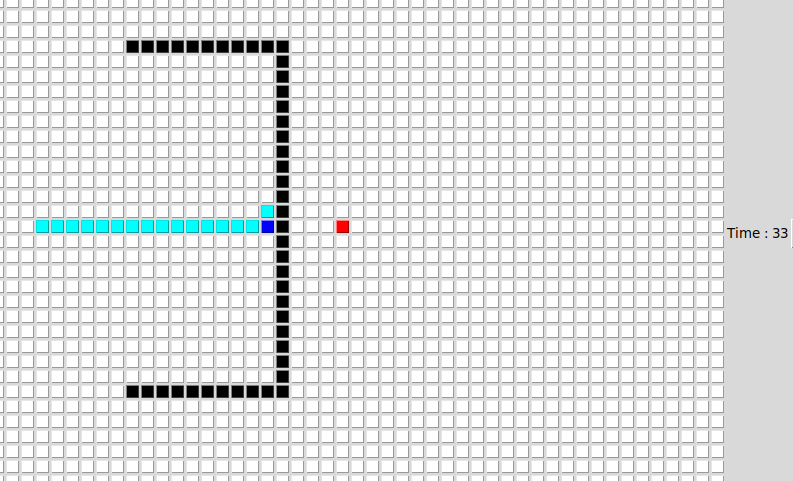
\includegraphics[height=4cm]{chicken_fail_blocked}
\newline \newline

To achieve this goal, the Dijkstra algorithm seems to be correct. The main idea is to initialize all cells with distance infinity (so here -1) and then assigne distances by neighboors.
In other terms, the distance is now the number of moves necessary to reach the target. One by one the neighboors to the cells distance x that are not obstacles take distance x+1. \newline \newline \newline

Therefore we started computing a distance matrix in a distance matrix function, that we would use to update one step function.
The first implementation of the the algorithm worked good to pass the chicken test and reach the target every time.
Nevertheless the problem was about the itinary. Our computation had the pedestrian use the minimum number of cells but not the direct line \newline \newline
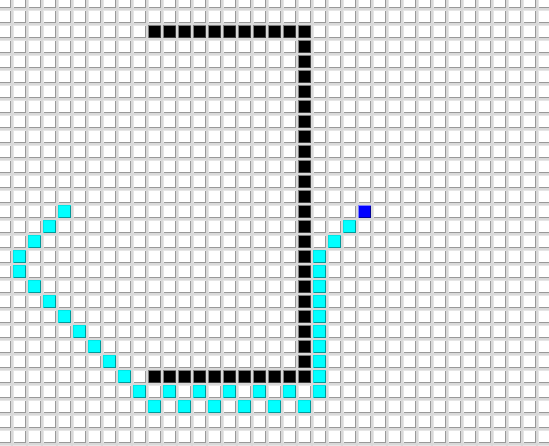
\includegraphics[height=3.7cm]{Dijk1}
~~~
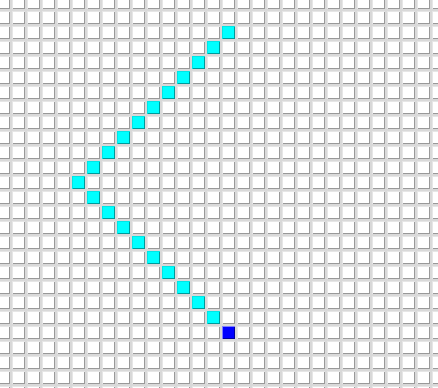
\includegraphics[height=3.7cm]{Dijk2} \newline 

To solve this problem we decided to try a mix between the euclidean distance and the Dijkstra distance. We added to our distance matrix function the computation of the euclidian matrix as a decimal (we divided the euclidean distance by twice the maximum possible euclidean distance between 2 cells and then sumed it to the Dijkstra distance). This way between 2 cells that are at the same distance from the target with Dijkstra, the euclidean distance would make the difference. This mostly solved the previous problems: \newline \newline
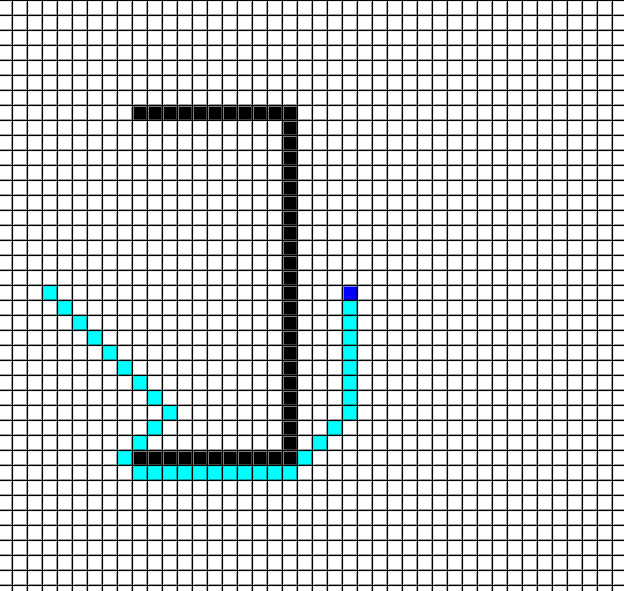
\includegraphics[height=3.8cm]{Prct1}
~~~
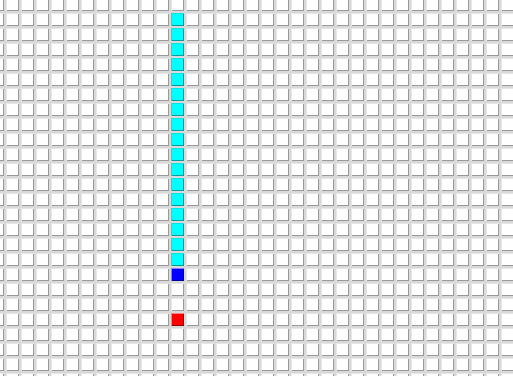
\includegraphics[height=3.8cm]{Dijk3} \newline 

Even though the Chicken test presented a slight deviation from the shortest path, because choosing between 2 cells it would take the closest to the target despite the fact that it might deviate a little from the obstacle, we decided that it was suffiscient for now, and that we would implement a change if it would become necessary in the tests (which it did not). One way of solving this would be a reconstruction of distance considering the effort of moving to go diagonal compared to straight, or maybe try an other algorithm like the Fast Marching one. \newline 

The next challenge was to deal with the corners issue. indeed the shortest way arround a corner is diagonal but that would mean scratching or even goign through the obstacle. It was then important to make sure the pedestrian would walk arround the corner. To do so, the main idea was to recompute the neighboors, such that when an obstacle was adjacent to a pedestrian, the diagonal next to the obstacle would not be considered as a neighboor anymore. To do so, we totally rebuilt the neighboors computation function, with checking every direct (non diagonal) neighboor and deleting the whole line if the cell was either out of boundaries or an obstacle. This solved the corner issue : \newline \newline
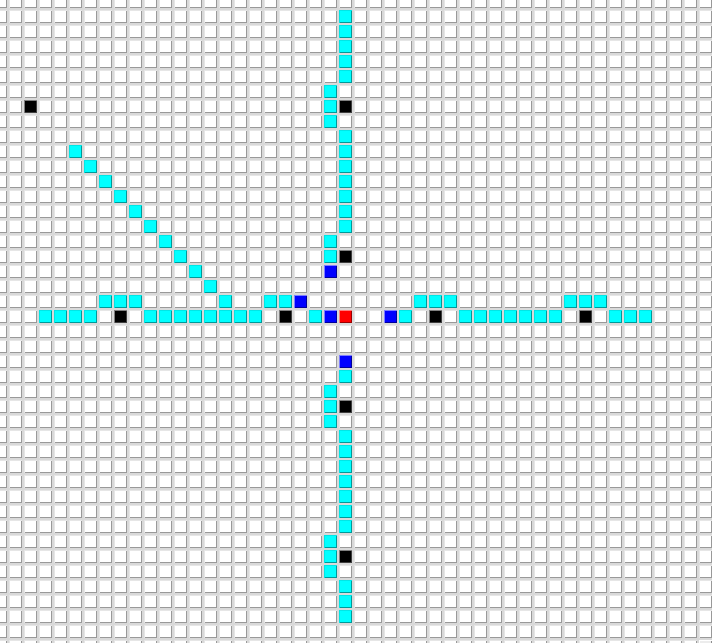
\includegraphics[height=3.8cm]{corner1}
~~~
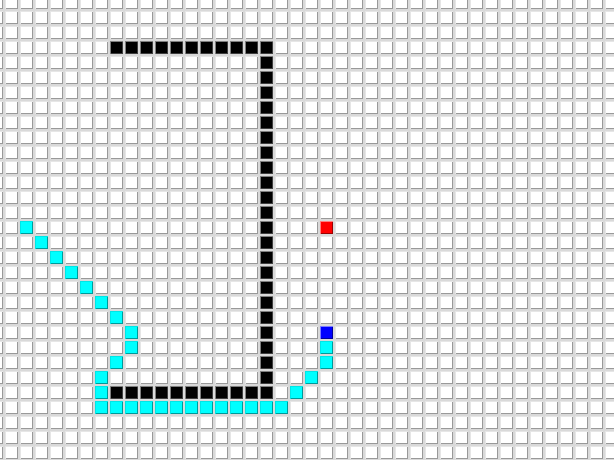
\includegraphics[height=3.8cm]{corner2} \newline \newline

\end{task}

\vfill\eject






\begin{task}{5/5, Tests}
.\newline\newline

After implementation of the first tasks in a pretty free environnment, now was time to test it on real conditions following a guideline of Rimea.\newline\newline

For the first test, we are set in a corridor of 40 meters long and 2 meters wide, with a speed of 1,33 m/s for one pedestrian of size 40cm*40cm, amd the test will play on the time to go from one end to the other of the corridor. \newline
We decided to stick with our previous model, setting the size of one cell 40cm*40cm. This way for this test the size of the grid would be 5*100 cells corresponding to the size of the corridor. \newline 

The challenge for this test was to implement the speed of a pedestrian, which we had not compute yet. In order to do so, 2 methods were tried: one step by step, keeping the the manual click corresponding to a certain time, the other one by adding a timer and a duration to have a real time simulation. \newline 

The second one used a real time simulation. Let's assume here that our pedestrian has a speed of 1,33 m/s, this means 3,33 cell/s. The idea of this implementation was to have - in this very example - our pedestrian move one cell every 0,3 second. To do so, a while loop was implemented comparing the current  time with the starting time. Every time the right amount of time was spent, the pedestrian would walk one step. \newline\newline
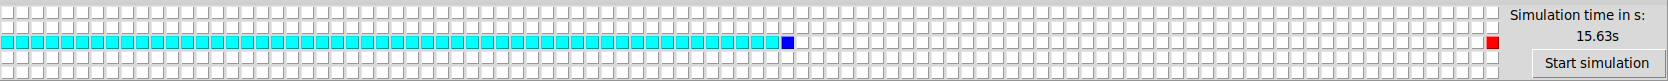
\includegraphics[height=0.9cm]{speed4} \newline \newline

The test was implemented for the test step by step with a time per click of 0,2s and thus a speed of 0,66 cell/click. The result was as followed: \newline \newline
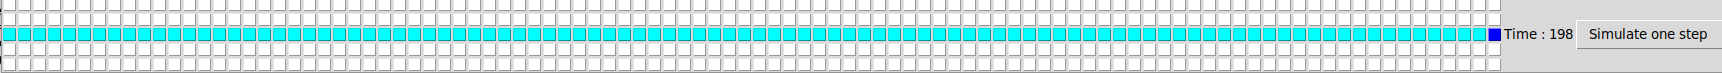
\includegraphics[height=0.78cm]{speed3}

The time necessary is thus 198*0,2 = 39,6s to cross the corridor, so more than 34s. The test was failed. \newline \newline

With the real time simulation with a duration of 40s, the result was as followed: \newline \newline
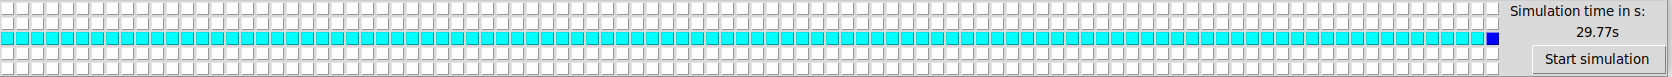
\includegraphics[height=0.86cm]{speed5}

The time necessary is thus 29,77s, which is correctly between 26s and 34s. The test was a success. \newline 

It happened the step by step methods had some flaws, but considering that we had a functional simulation, we decided to keep the second simulation, in real time, for the next tests. \newline

 The test 1 anyway was passed this way. \vfill\eject

The test 2 ......... \vfill\eject

For the third test, the implementation required to put 20 people in a corridor and have them pass a corner. We kept a speed of 1,33m/s for each pedestrian and put them in the entrance of the corridor. \newline \newline

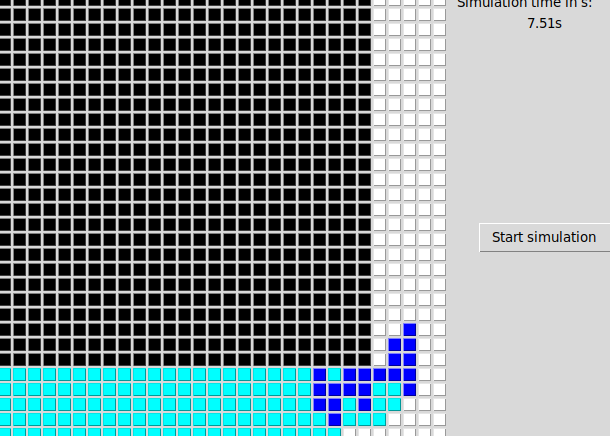
\includegraphics[height=6cm]{corner11}
~~~
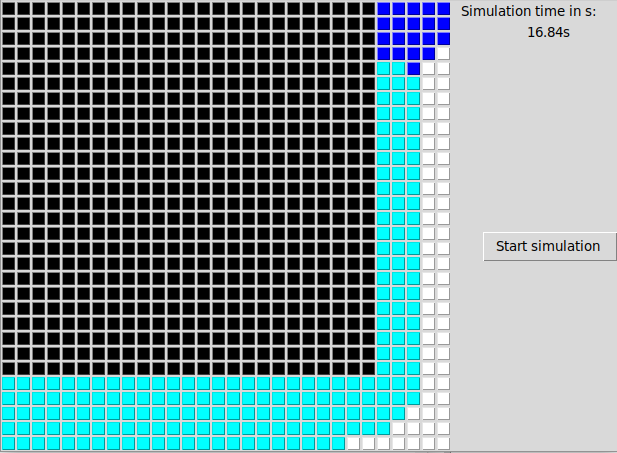
\includegraphics[height=6cm]{corner12} \newline \newline

It is clear on the first image that the pedestrians do not cut the edges of the corner, and in the second picture we see that all of them did cross the corner in a normal time. \newline \newline

The test 3 is passed


 \vfill\eject

The test 4 .......

\end{task}


\bibliographystyle{plain}
\bibliography{Literature}

\end{document}